\documentclass{note}
%\addtolength{\topmargin}{-2cm}
%\addtolength{\textheight}{2cm}
\usepackage{mathptm,mydef}
%\usepackage{courier}
%\renewcommand{\ttdefault}{txtt}
\usepackage[all]{xy}
%\usepackage{MinionPro}

\usepackage{graphicx}
\usepackage{alltt}
\usepackage[T1]{fontenc}
\DeclareGraphicsExtensions{.png,.jpg}

\usepackage{hyperref}
\hypersetup{
    colorlinks, 
    citecolor=black, 
    filecolor=black, 
    linkcolor=blue, 
    urlcolor=black
}

\begin{document}
\small


\begin{center}
 {\large\bf Scala, Akka, and Actors: Overview}
\end{center}

\vspace*{1cm}

\tableofcontents

\section{Actors}
\bit
\w an \bb{actor} is an object which encapsulate \bb{state} and \bb{behavior}
\w communication between actors are exclusively by exchanging messages which
are placed into the recipient's mailbox
\w \bb{hierarchy of actors}:
   \bit
   \w an actor can \bb{supervise} child actors
   \w each actor has exactly only one \bb{supervisor}
   \eit
\w \bb{actor best practices}
  \bit
  \w do not pass \textcolor{red}{\bf{}mutable objects} between actors --
  prefer \bb{immutable messages}
  \w actors are made to be containers for beahvior and state
     \bit
     \w try NOT to send ``behavior'' within messages (tempting -- e.g. process
     migration) but may be very difficult to debug, etc.
     \eit
  \w top-level actors are expensive -- try to minimize their numbers
  \eit
\w \bb{supervisor}
   \bit
   \w supervisor (parent) delegates tasks to subordinates (child)
   \w \bb{when child fails, parent must handle the failure}
      \bit
      \w when failure; suspend itself and all its subordinates; sends a
      message to parent; signaling parent of failure
      \eit
   \eit
\w \bb{actor reference}: subtype of \verb+ActorRef+
  \bit
  \w purpose: support sending meessages to the actor it represents
  \w each actor has its local reference through \verb+self+
  \w each receptor can access sender's reference by \verb+sender+ field
  \w \verb+Router inherits ActorRef+
     \bit
     \w sending message to \verb+Router+ will cause its message to be routed
       to children of the ``Router''
     \eit
  \eit
\w \bb{actor path}:
    since actors are created in hierarchical fashion, actor names can be given
    in a hier-path
   \bit
   \w \verb+"[ActorSystem]://[RootGuardian]/actor1/actor2"+
\begin{verbatim}
"akka://my-sys/user/service-a/worker1" // purely local
"akka.tcp://my-sys@host.example.com:5678/user/service-b" // remote
"cluster://my-cluster/service-c" // clustered (Future Extension)
\end{verbatim}
   \eit

\w \textcolor{red}{\bf{}OBTAINING Actor references}
  \bit
  \w \bb{creating actors}
\begin{verbatim}
  ActorSystem.actorOf
  ActorContext.actorOf
\end{verbatim}
  \w \bb{looking up actors by concrete path}
\begin{verbatim}
  ActorSystem.actorSelection

  context.actorSelection("../brother") ! msg
  context.actorSelection("/usr/serviceA") ! msg
\end{verbatim}
  \eit
\eit


\centerline{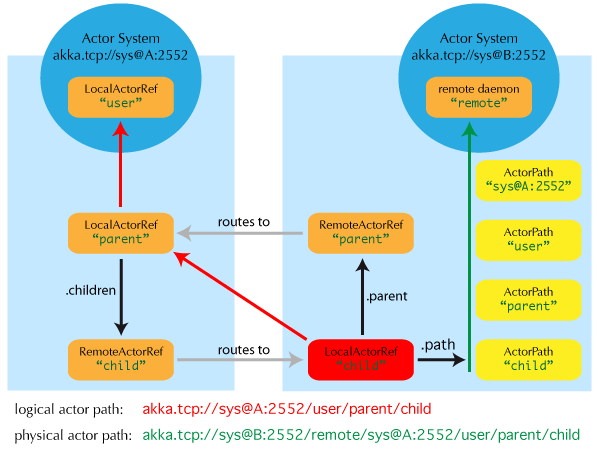
\includegraphics[width=8cm]{pics/remote-deployment}}

\section{Actors and Java Memory Model}
\bit
\w two ways multiple threads can execute actions on shared memory
  (in Actors implementation in Akka)
\bit
\w \bb{if a message is sent to an actor (e.g. by another actor)}. In most cases
messages are immutable, but if that message is not a properly constructed
immutable object, without a ``happens-before'' rule, it would be
possible for the receiver to see partially initialized data structures and
possibly even values out of thin air (longs/doubles).

\w  \bb{if an actor makes changes to its internal state while processing a
message, and accesses that state while 
processing another message moments later}: It is important to realize that with the actor model you don't get
any guarantee that the same thread will be executing the same actor for
different messages.
\eit
To prevent visibility and reordering problems on actors, Akka guarantees the following two ``happens before''
rules:
\bit
\w  \bb{The actor send rule}: the send of the message to an actor happens before the receive of that message by the
same actor.
\w \bb{The actor subsequent processing rule}: processing of one message happens before processing of the next
message by the same actor. 
\eit
\eit

\section{Typing in Actors}
\bit
\w \bb{messages} are strongly-typed
\w \bb{endpoints, i.e. actors} are loosely-typed
   \bit
   \w  every actor look like every other actor
   \w they may behave differently or may accept a different set of messages
   \w AKKA also supports \bb{typed actors}
   \eit
\w \bb{EXAMPLE: WEB SERVICE}
   \bit
   \w web servers are untyped as well (endpoints are untyped)
   \w they are just HTTP-servers
   \w ``messages -- payload'' ``distinguishes''
   \eit
\eit

\section{Actors and Futures}
\bit
\w send ``request'' messages
\w WE DON'T KNOW WHEN THE RESPONSE WILL ARRIVE
\w add FUTURE which will be executed upon RESPONSE
\eit

\end{document}
